\documentclass[10pt]{article}
\usepackage{tikz}
\usetikzlibrary{shapes.misc}
\usepackage[margin=0cm]{geometry}
\pagestyle{empty}
\tikzstyle{every node}=[cross out, draw, red]

\begin{document}

\vspace*{\fill}
\begin{center}
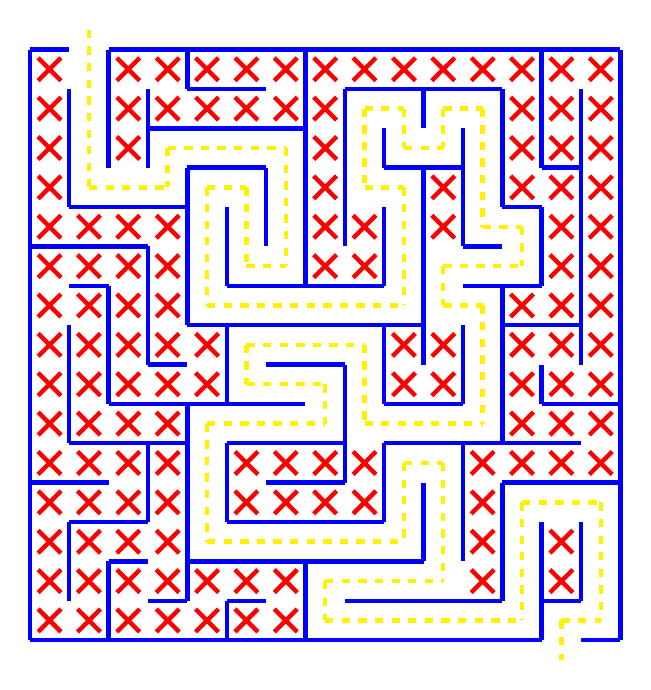
\begin{tikzpicture}[x=0.5cm, y=-0.5cm, ultra thick, blue]
% Walls
    \draw (0,0) -- (1,0);
    \draw (2,0) -- (15,0);
    \draw (4,1) -- (6,1);
    \draw (8,1) -- (12,1);
    \draw (3,2) -- (7,2);
    \draw (4,3) -- (6,3);
    \draw (9,3) -- (11,3);
    \draw (13,3) -- (14,3);
    \draw (1,4) -- (4,4);
    \draw (12,4) -- (13,4);
    \draw (0,5) -- (3,5);
    \draw (11,5) -- (12,5);
    \draw (1,6) -- (2,6);
    \draw (5,6) -- (9,6);
    \draw (11,6) -- (13,6);
    \draw (4,7) -- (10,7);
    \draw (12,7) -- (14,7);
    \draw (3,8) -- (4,8);
    \draw (6,8) -- (8,8);
    \draw (2,9) -- (7,9);
    \draw (9,9) -- (11,9);
    \draw (13,9) -- (15,9);
    \draw (1,10) -- (4,10);
    \draw (5,10) -- (8,10);
    \draw (9,10) -- (14,10);
    \draw (0,11) -- (2,11);
    \draw (6,11) -- (8,11);
    \draw (12,11) -- (15,11);
    \draw (1,12) -- (3,12);
    \draw (5,12) -- (9,12);
    \draw (2,13) -- (3,13);
    \draw (4,13) -- (10,13);
    \draw (3,14) -- (4,14);
    \draw (5,14) -- (6,14);
    \draw (8,14) -- (12,14);
    \draw (13,14) -- (14,14);
    \draw (0,15) -- (13,15);
    \draw (14,15) -- (15,15);
    \draw (0,0) -- (0,15);
    \draw (1,1) -- (1,4);
    \draw (1,7) -- (1,10);
    \draw (1,12) -- (1,14);
    \draw (2,0) -- (2,3);
    \draw (2,6) -- (2,9);
    \draw (2,13) -- (2,15);
    \draw (3,1) -- (3,3);
    \draw (3,5) -- (3,8);
    \draw (3,10) -- (3,12);
    \draw (4,0) -- (4,1);
    \draw (4,3) -- (4,7);
    \draw (4,9) -- (4,14);
    \draw (5,4) -- (5,6);
    \draw (5,7) -- (5,9);
    \draw (5,10) -- (5,12);
    \draw (5,14) -- (5,15);
    \draw (6,3) -- (6,5);
    \draw (7,0) -- (7,6);
    \draw (7,13) -- (7,15);
    \draw (8,1) -- (8,5);
    \draw (8,8) -- (8,11);
    \draw (9,2) -- (9,3);
    \draw (9,4) -- (9,6);
    \draw (9,7) -- (9,9);
    \draw (9,10) -- (9,12);
    \draw (10,1) -- (10,2);
    \draw (10,3) -- (10,8);
    \draw (10,11) -- (10,13);
    \draw (11,2) -- (11,5);
    \draw (11,7) -- (11,9);
    \draw (11,10) -- (11,13);
    \draw (12,1) -- (12,4);
    \draw (12,6) -- (12,10);
    \draw (12,11) -- (12,14);
    \draw (13,0) -- (13,3);
    \draw (13,4) -- (13,6);
    \draw (13,8) -- (13,9);
    \draw (13,12) -- (13,15);
    \draw (14,1) -- (14,8);
    \draw (14,12) -- (14,14);
    \draw (15,0) -- (15,15);
% Pillars
% Inner points in accessible cul-de-sacs
    \node at (0.5,0.5) {};
    \node at (2.5,0.5) {};
    \node at (3.5,0.5) {};
    \node at (4.5,0.5) {};
    \node at (5.5,0.5) {};
    \node at (6.5,0.5) {};
    \node at (7.5,0.5) {};
    \node at (8.5,0.5) {};
    \node at (9.5,0.5) {};
    \node at (10.5,0.5) {};
    \node at (11.5,0.5) {};
    \node at (12.5,0.5) {};
    \node at (13.5,0.5) {};
    \node at (14.5,0.5) {};
    \node at (0.5,1.5) {};
    \node at (2.5,1.5) {};
    \node at (3.5,1.5) {};
    \node at (4.5,1.5) {};
    \node at (5.5,1.5) {};
    \node at (6.5,1.5) {};
    \node at (7.5,1.5) {};
    \node at (12.5,1.5) {};
    \node at (13.5,1.5) {};
    \node at (14.5,1.5) {};
    \node at (0.5,2.5) {};
    \node at (2.5,2.5) {};
    \node at (7.5,2.5) {};
    \node at (12.5,2.5) {};
    \node at (13.5,2.5) {};
    \node at (14.5,2.5) {};
    \node at (0.5,3.5) {};
    \node at (7.5,3.5) {};
    \node at (10.5,3.5) {};
    \node at (12.5,3.5) {};
    \node at (13.5,3.5) {};
    \node at (14.5,3.5) {};
    \node at (0.5,4.5) {};
    \node at (1.5,4.5) {};
    \node at (2.5,4.5) {};
    \node at (3.5,4.5) {};
    \node at (7.5,4.5) {};
    \node at (8.5,4.5) {};
    \node at (10.5,4.5) {};
    \node at (13.5,4.5) {};
    \node at (14.5,4.5) {};
    \node at (0.5,5.5) {};
    \node at (1.5,5.5) {};
    \node at (2.5,5.5) {};
    \node at (3.5,5.5) {};
    \node at (7.5,5.5) {};
    \node at (8.5,5.5) {};
    \node at (13.5,5.5) {};
    \node at (14.5,5.5) {};
    \node at (0.5,6.5) {};
    \node at (1.5,6.5) {};
    \node at (2.5,6.5) {};
    \node at (3.5,6.5) {};
    \node at (12.5,6.5) {};
    \node at (13.5,6.5) {};
    \node at (14.5,6.5) {};
    \node at (0.5,7.5) {};
    \node at (1.5,7.5) {};
    \node at (2.5,7.5) {};
    \node at (3.5,7.5) {};
    \node at (4.5,7.5) {};
    \node at (9.5,7.5) {};
    \node at (10.5,7.5) {};
    \node at (12.5,7.5) {};
    \node at (13.5,7.5) {};
    \node at (14.5,7.5) {};
    \node at (0.5,8.5) {};
    \node at (1.5,8.5) {};
    \node at (2.5,8.5) {};
    \node at (3.5,8.5) {};
    \node at (4.5,8.5) {};
    \node at (9.5,8.5) {};
    \node at (10.5,8.5) {};
    \node at (12.5,8.5) {};
    \node at (13.5,8.5) {};
    \node at (14.5,8.5) {};
    \node at (0.5,9.5) {};
    \node at (1.5,9.5) {};
    \node at (2.5,9.5) {};
    \node at (3.5,9.5) {};
    \node at (12.5,9.5) {};
    \node at (13.5,9.5) {};
    \node at (14.5,9.5) {};
    \node at (0.5,10.5) {};
    \node at (1.5,10.5) {};
    \node at (2.5,10.5) {};
    \node at (3.5,10.5) {};
    \node at (5.5,10.5) {};
    \node at (6.5,10.5) {};
    \node at (7.5,10.5) {};
    \node at (8.5,10.5) {};
    \node at (11.5,10.5) {};
    \node at (12.5,10.5) {};
    \node at (13.5,10.5) {};
    \node at (14.5,10.5) {};
    \node at (0.5,11.5) {};
    \node at (1.5,11.5) {};
    \node at (2.5,11.5) {};
    \node at (3.5,11.5) {};
    \node at (5.5,11.5) {};
    \node at (6.5,11.5) {};
    \node at (7.5,11.5) {};
    \node at (8.5,11.5) {};
    \node at (11.5,11.5) {};
    \node at (0.5,12.5) {};
    \node at (1.5,12.5) {};
    \node at (2.5,12.5) {};
    \node at (3.5,12.5) {};
    \node at (11.5,12.5) {};
    \node at (13.5,12.5) {};
    \node at (0.5,13.5) {};
    \node at (1.5,13.5) {};
    \node at (2.5,13.5) {};
    \node at (3.5,13.5) {};
    \node at (4.5,13.5) {};
    \node at (5.5,13.5) {};
    \node at (6.5,13.5) {};
    \node at (11.5,13.5) {};
    \node at (13.5,13.5) {};
    \node at (0.5,14.5) {};
    \node at (1.5,14.5) {};
    \node at (2.5,14.5) {};
    \node at (3.5,14.5) {};
    \node at (4.5,14.5) {};
    \node at (5.5,14.5) {};
    \node at (6.5,14.5) {};
% Entry-exit paths without intersections
    \draw[dashed, yellow] (8.5,1.5) -- (9.5,1.5);
    \draw[dashed, yellow] (10.5,1.5) -- (11.5,1.5);
    \draw[dashed, yellow] (3.5,2.5) -- (6.5,2.5);
    \draw[dashed, yellow] (9.5,2.5) -- (10.5,2.5);
    \draw[dashed, yellow] (1.5,3.5) -- (3.5,3.5);
    \draw[dashed, yellow] (4.5,3.5) -- (5.5,3.5);
    \draw[dashed, yellow] (8.5,3.5) -- (9.5,3.5);
    \draw[dashed, yellow] (11.5,4.5) -- (12.5,4.5);
    \draw[dashed, yellow] (5.5,5.5) -- (6.5,5.5);
    \draw[dashed, yellow] (10.5,5.5) -- (12.5,5.5);
    \draw[dashed, yellow] (4.5,6.5) -- (9.5,6.5);
    \draw[dashed, yellow] (10.5,6.5) -- (11.5,6.5);
    \draw[dashed, yellow] (5.5,7.5) -- (8.5,7.5);
    \draw[dashed, yellow] (5.5,8.5) -- (7.5,8.5);
    \draw[dashed, yellow] (4.5,9.5) -- (7.5,9.5);
    \draw[dashed, yellow] (8.5,9.5) -- (11.5,9.5);
    \draw[dashed, yellow] (9.5,10.5) -- (10.5,10.5);
    \draw[dashed, yellow] (12.5,11.5) -- (14.5,11.5);
    \draw[dashed, yellow] (4.5,12.5) -- (9.5,12.5);
    \draw[dashed, yellow] (7.5,13.5) -- (10.5,13.5);
    \draw[dashed, yellow] (7.5,14.5) -- (12.5,14.5);
    \draw[dashed, yellow] (13.5,14.5) -- (14.5,14.5);
    \draw[dashed, yellow] (1.5,-0.5) -- (1.5,3.5);
    \draw[dashed, yellow] (3.5,2.5) -- (3.5,3.5);
    \draw[dashed, yellow] (4.5,3.5) -- (4.5,6.5);
    \draw[dashed, yellow] (4.5,9.5) -- (4.5,12.5);
    \draw[dashed, yellow] (5.5,3.5) -- (5.5,5.5);
    \draw[dashed, yellow] (5.5,7.5) -- (5.5,8.5);
    \draw[dashed, yellow] (6.5,2.5) -- (6.5,5.5);
    \draw[dashed, yellow] (7.5,8.5) -- (7.5,9.5);
    \draw[dashed, yellow] (7.5,13.5) -- (7.5,14.5);
    \draw[dashed, yellow] (8.5,1.5) -- (8.5,3.5);
    \draw[dashed, yellow] (8.5,7.5) -- (8.5,9.5);
    \draw[dashed, yellow] (9.5,1.5) -- (9.5,2.5);
    \draw[dashed, yellow] (9.5,3.5) -- (9.5,6.5);
    \draw[dashed, yellow] (9.5,10.5) -- (9.5,12.5);
    \draw[dashed, yellow] (10.5,1.5) -- (10.5,2.5);
    \draw[dashed, yellow] (10.5,5.5) -- (10.5,6.5);
    \draw[dashed, yellow] (10.5,10.5) -- (10.5,13.5);
    \draw[dashed, yellow] (11.5,1.5) -- (11.5,4.5);
    \draw[dashed, yellow] (11.5,6.5) -- (11.5,9.5);
    \draw[dashed, yellow] (12.5,4.5) -- (12.5,5.5);
    \draw[dashed, yellow] (12.5,11.5) -- (12.5,14.5);
    \draw[dashed, yellow] (13.5,14.5) -- (13.5,15.5);
    \draw[dashed, yellow] (14.5,11.5) -- (14.5,14.5);
\end{tikzpicture}
\end{center}
\vspace*{\fill}

\end{document}
